\chapter{LLM Biases in Bayesian Diagnostic Reasoning} \label{chapter:race-bayes}

\section{Introduction}

\begin{wrapfigure}{r}{0.65\textwidth}
	\centering
	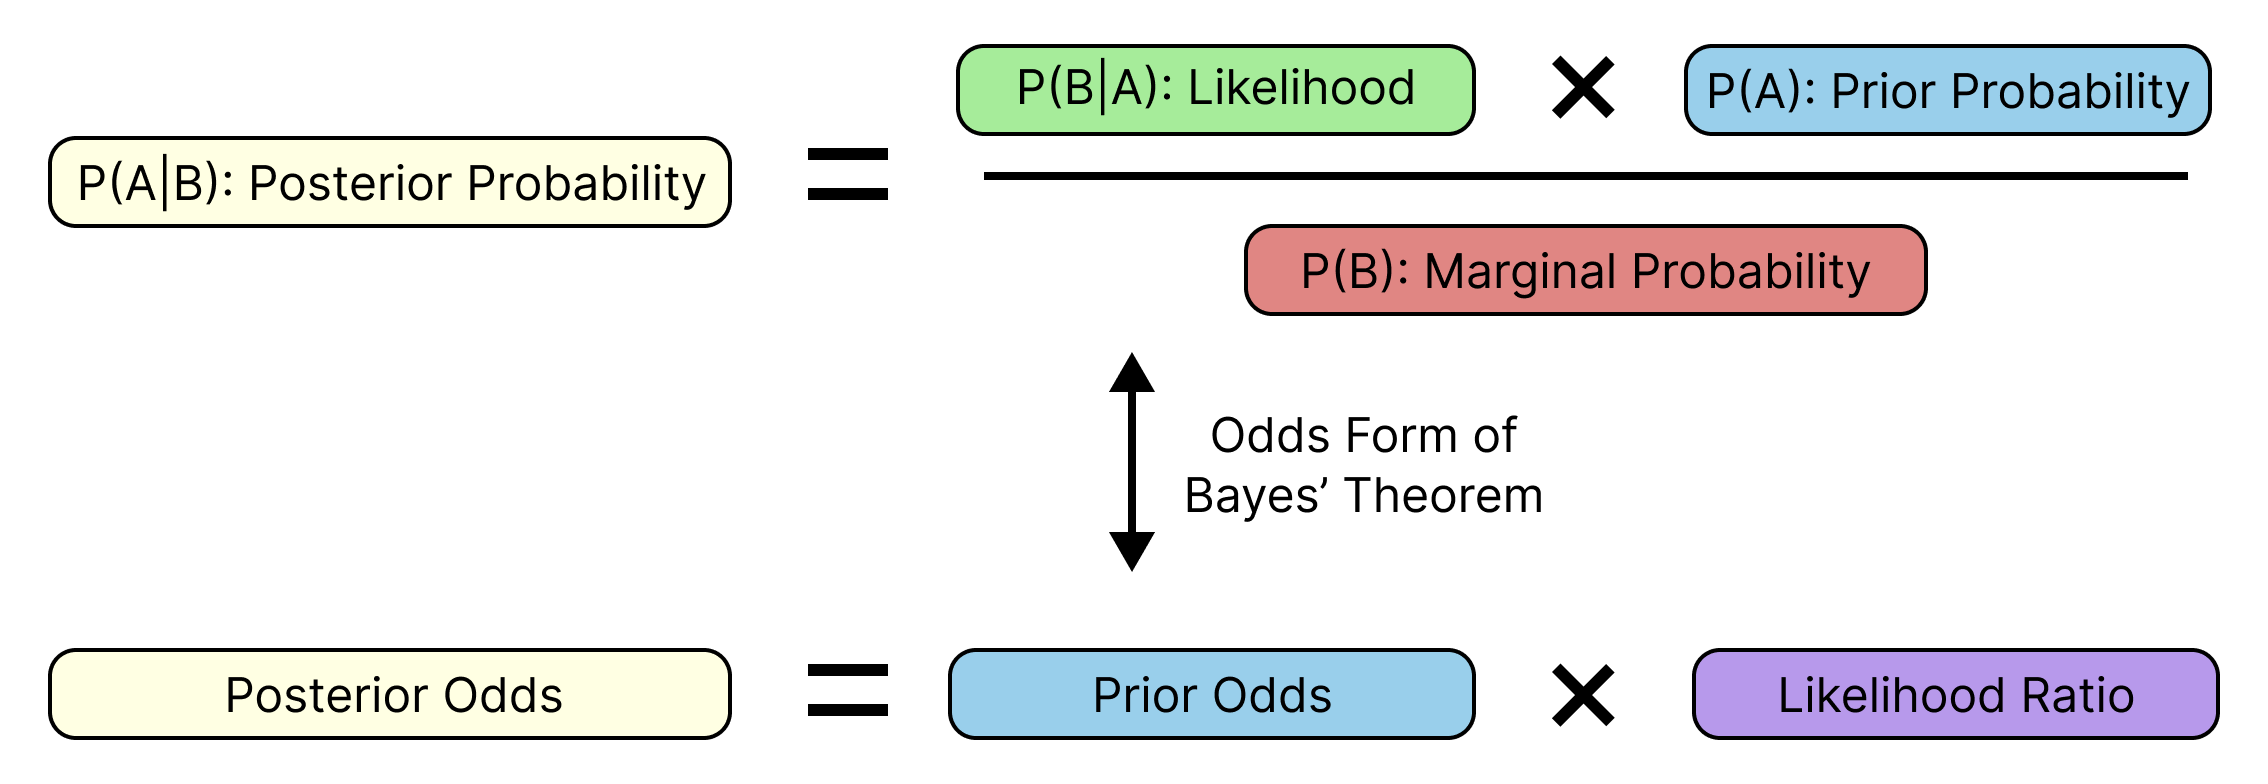
\includegraphics[width=0.6\textwidth] {figures/aim2/Figure1.png}
	\caption{Estimated likelihood ratios calculated from estimated sensitivity and specificity for GPT 4o-mini and GPT 4o. Dashed horizontal red line identifies the likelihood ratio from Brush et al. Temperature was varied for GPT 4o between 0.8 and 0.0 (deterministic prediction). Error bars represent ± one standard error from the mean.} \label{fig:aim2-bayesrule}
\end{wrapfigure}

The interpretation of diagnostic testing is a central component of clinical decision making. Diagnostic testing is the single most performed medical activity, with more than half of all clinical decisions made on the basis of laboratory testing\citep{brucealexanderMessagePresidentReducing2012, zhiLandscapeInappropriateLaboratory2013}. A clear understanding of test characteristics is vital in both reducing healthcare expenditures and improving overall quality of care for patients\citep{dugganWhyPretestProbability2020, reedPretestProbabilityShould2013}. Classical diagnostic reasoning involves updating initial estimates of disease likelihood as diagnostic testing is ordered and results are returned. This process can be modeled through Bayes’ rule (Figure \ref{fig:aim2-bayesrule})\citep{boursBayesRuleDiagnosis2021}. Unfortunately, significant evidence suggests that physicians are inaccurate in their estimates of disease probabilities and test characteristics, often falling for cognitive biases\citep{cahanProbabilisticReasoningClinical2003, hallEstimationPosttestProbabilities2014, manraiMedicinesUncomfortableRelationship2014, morganAccuracyPractitionerEstimates2021, normanCausesErrorsClinical2017}.

Large language models (LLMs) have been shown to effectively perform numerical reasoning in a variety of settings\citep{imaniMathPrompterMathematicalReasoning2023, lewkowyczSolvingQuantitativeReasoning2024}. A recent study examined GPT-4’s ability to estimate disease probabilities via Bayes’ rule across four patient vignettes, demonstrating that the LLM was comparable to physicians for estimating post-test probability after a positive diagnostic test\citep{clusmannFutureLandscapeLarge2023}. However, this study did not utilize advanced prompting techniques such as chain-of-thought reasoning\citep{rodmanArtificialIntelligenceVs2023}, nor did it allow classification of LLM reasoning error modes (i.e. misestimating the sensitivity/specificity of diagnostic tests, incorrectly applying Bayes’ rule, etc.). Advanced prompting strategies such as CoT have been shown to significantly improve reasoning in LLMs, allowing us to test the full capabilities of both models\citep{weiChainthoughtPromptingElicits2024}. Moreover, prior work has demonstrated that disease categories impact LLM performance\citep{thirunavukarasuTriallingLargeLanguage2023}. Disease-specific variability in LLM risk estimation remains underexplored due to the previous study’s use of single vignettes for evaluating each clinical context\citep{morganAccuracyPractitionerEstimates2021}. Finally, while LLMs have the potential to better estimate disease probability, there is concern that they will further exacerbate health inequities due to hidden sociodemographic biases arising from training data\citep{clusmannFutureLandscapeLarge2023, liEthicsLargeLanguage2023, zackAssessingPotentialGPT42024, nastasiVignettebasedEvaluationChatGPTs2023}. Despite initial work done in evaluating the impact of LLMs’ biases on clinical decision making, previous studies have not evaluated how these biases may impact diagnostics, such as in a clinical decision support tool. In this work, we focus on race, as other demographics (e.g. age, gender) may  influence disease prevalence in our vignettes, potentially complicating the interpretation of post-test probability errors.

Our work aims to expand on previous research by evaluating both disease variation and racial biases in estimating risk through a Bayesian diagnostic framework by two state-of-the-art LLMs of different reasoning capabilities: GPT 4o-mini and GPT 4o. By modifying the availability of likelihood ratio information, we seek to identify specific points in the reasoning process that influence error in risk estimation. To investigate potential biases in the diagnostic risk assessments of these LLMs, we evaluate several vignettes across 4 distinct conditions and systematically vary race throughout our evaluation.

\section{Methods}

\subsection{Vignette Selection}

To evaluate the impacts of disease and race on Bayesian reasoning in LLMs, we gathered clinical vignettes from four common ED presentations with clearly defined diagnostic tests and validated positive and negative likelihood ratios (LRs). We chose previously developed vignettes from \citet{brushEffectTeachingBayesian2019}. The vignettes included clinical presentations, history, physical exam findings, as well as vitals and lab values when relevant. A total of 43 vignettes were used, covering 4 ED diagnoses: acute coronary syndrome (ACS), congestive heart failure (CHF), pneumonia, and pulmonary embolism (PE). Each vignette was also accompanied by a relevant laboratory test or radiologic study that was conducted following the initial presentation. 

Originally designed to assess Bayesian reasoning in medical students, each vignette begins by asking for an initial pre-test probability of disease on a scale from 0 to 100\%. After determining the pre-test probability, participants were given the results of the diagnostic test, reported as either positive or negative, along with literature-validated data on sensitivity, specificity, and positive and negative LRs. Finally, participants used the initial presentation and test results to estimate a post-test probability of disease. We adapted these vignettes to require the LLM to estimate sensitivity and specificity, rather than relying on literature-derived values from Brush et al., allowing for a more fine-grained evaluation of its reasoning process. We selected vignettes that were physiologically likely, regardless of race for our racial bias evaluation. A description of the vignettes is shown in Table 1.

\begin{table}
\caption{Description of vignette diagnoses and relevant lab tests. Literature-derived diagnostic accuracy characteristics come from \citet{brushEffectTeachingBayesian2019}}
\label{tab:aim2-vignettes}
\begin{tabular}{llc} \toprule
Diagnosis & Lab Test & Number of vignettes \\ \midrule
Acute Coronary Syndrome (ACS) & Troponin I & 13 \\
Congestive Heart Failure (CHF) & Chest X-ray & 13 \\
Pneumonia & Chest X-ray & 4 \\
Pulmonary Embolism (PE) & Quantitative D-dimer & 13 \\ \bottomrule
\end{tabular}%
\end{table}

\subsection{Bias Dimensions}

To assess the impact of disease-specific bias, we evaluate LLM responses over all vignettes within a disease category. Specifically, we average post-test probability error rates, defined in the next section, over all vignettes associated with a specific disease. To assess the impact of racial bias on risk estimation, we vary race in the history of present illness (HPI) component of the vignette using the U.S. Department of the Interior racial categories: American Indian or Alaska Native, Asian, Black or African American, Hispanic or Latino, Native Hawaiian or Other Pacific Islander, and White.

\subsection{Bias-Aware Diagnostic Reasoning Evaluation}

We conducted all experiments through Azure OpenAI using both GPT 4o and GPT 4o-mini, employing prompts specifying CoT. We generate a distribution of disease probability estimates for a given vignette by repeating each vignette 10 times with GPT 4o-mini and 5 times with GPT 4o for both positive and negative test results with high temperature (0.8, [range: 0-1]). Due to budget constraints, repeated trials of GPT-4o were limited because of the large number of combinations involving the vignettes, test results, and race. The high temperature ensures that the LLM generates different responses for each trial, allowing us to characterize the full range of probability estimates an LLM might generate\citep{openaiGPT4TechnicalReport2024}.

We evaluate performance of both LLMs by computing the post-test probability error, defined as the difference between the true post-test probability, computed using the estimated pre-test probability and literature-derived likelihood ratios, and the estimated post-test probability generated from the LLM. The estimated pre-test probability is assumed to be valid, acknowledging that prevalence can depend on various factors such as geographic location and presenting signs or symptoms. Consequently, our focus is on evaluating the models' capacity for Bayesian reasoning rather than their ability to estimate initial clinical disease risk. We also compute the estimated likelihood ratios from estimated sensitivity and specificity, and compare these to the provided LRs in \citet{brushEffectTeachingBayesian2019} 

To estimate post-test probability, likelihood ratio information was provided to the models under three conditions. In Condition 1, we assessed the implicit estimation of disease risk by having the models estimate post-test probabilities following test results without any likelihood ratio information or explicit references to Bayesian reasoning. This condition evaluated the models' ability to infer disease risk without external Bayesian guidance. In Condition 2, the LLMs estimated the sensitivity and specificity of the diagnostic test given an initial patient presentation. The models then used their estimated likelihood ratios to predict post-test risk, encouraging Bayesian reasoning while still limiting external information. Finally, in Condition 3 (the baseline), we provided the LLMs with literature-derived likelihood ratios from Brush et al., enabling the assessment of diagnostic reasoning with full, explicit Bayesian information. This approach allowed for the evaluation of the models’ performance under implicit, partial, and full Bayesian conditions.

Finally, to examine racial bias, for each vignette, we alter the patient’s race in the HPI. Given the repeated trials described above, this yields a total of 5,160 for GPT 4o-mini and 2,580 runs for GPT 4o. In addition to estimating disease probability distributions, we hypothesize that differences in diagnostic accuracy are inherent biases baked into the models from training data, not a function of their stochasticity, so we repeat LR estimation in a near-deterministic setting (temperature=0.0; random seed=314). All results were reported with ± 1 standard error from the mean using Python 3.10, scipy\citep{virtanenSciPy10Fundamental2020} for statistical analysis, and seaborn\citep{waskomSeabornStatisticalData2021} for data visualization. 

\section{Results}

In Figure 2, we present the post-test probability error of GPT 4o-mini and GPT 4o with three elements of likelihood ratio information: none, estimated, and true LRs. Across all disease conditions, GPT 4o-mini estimated disease risk more accurately when given either estimated (post-test prob. error: -1.75 ±19.69) or literature-derived LRs (0.38 ± 8.22), compared to when the model estimated risk with implicit Bayesian reasoning (4.01 ± 24.29). This trend was also evident in GPT 4o, but with even greater accuracy when provided literature-derived LRs (0.02 ± 0.52). Both models variably demonstrated under- or overestimation of disease risk by disease condition. For instance, both models significantly overestimated ACS risk, regardless of Troponin results when no LRs were provided (GPT 4o-mini: -3.50 ± 32.72, GPT 4o: -14.66 ± 19.68). Unlike the variation observed due to disease category, post-test probability errors did not differ significantly by race (one-way ANOVA p-values across diseases: GPT-4o, p = 0.66–1.00; GPT-4o-mini, p = 0.72–1.00).

\begin{figure}[!htbp]
	\centering
	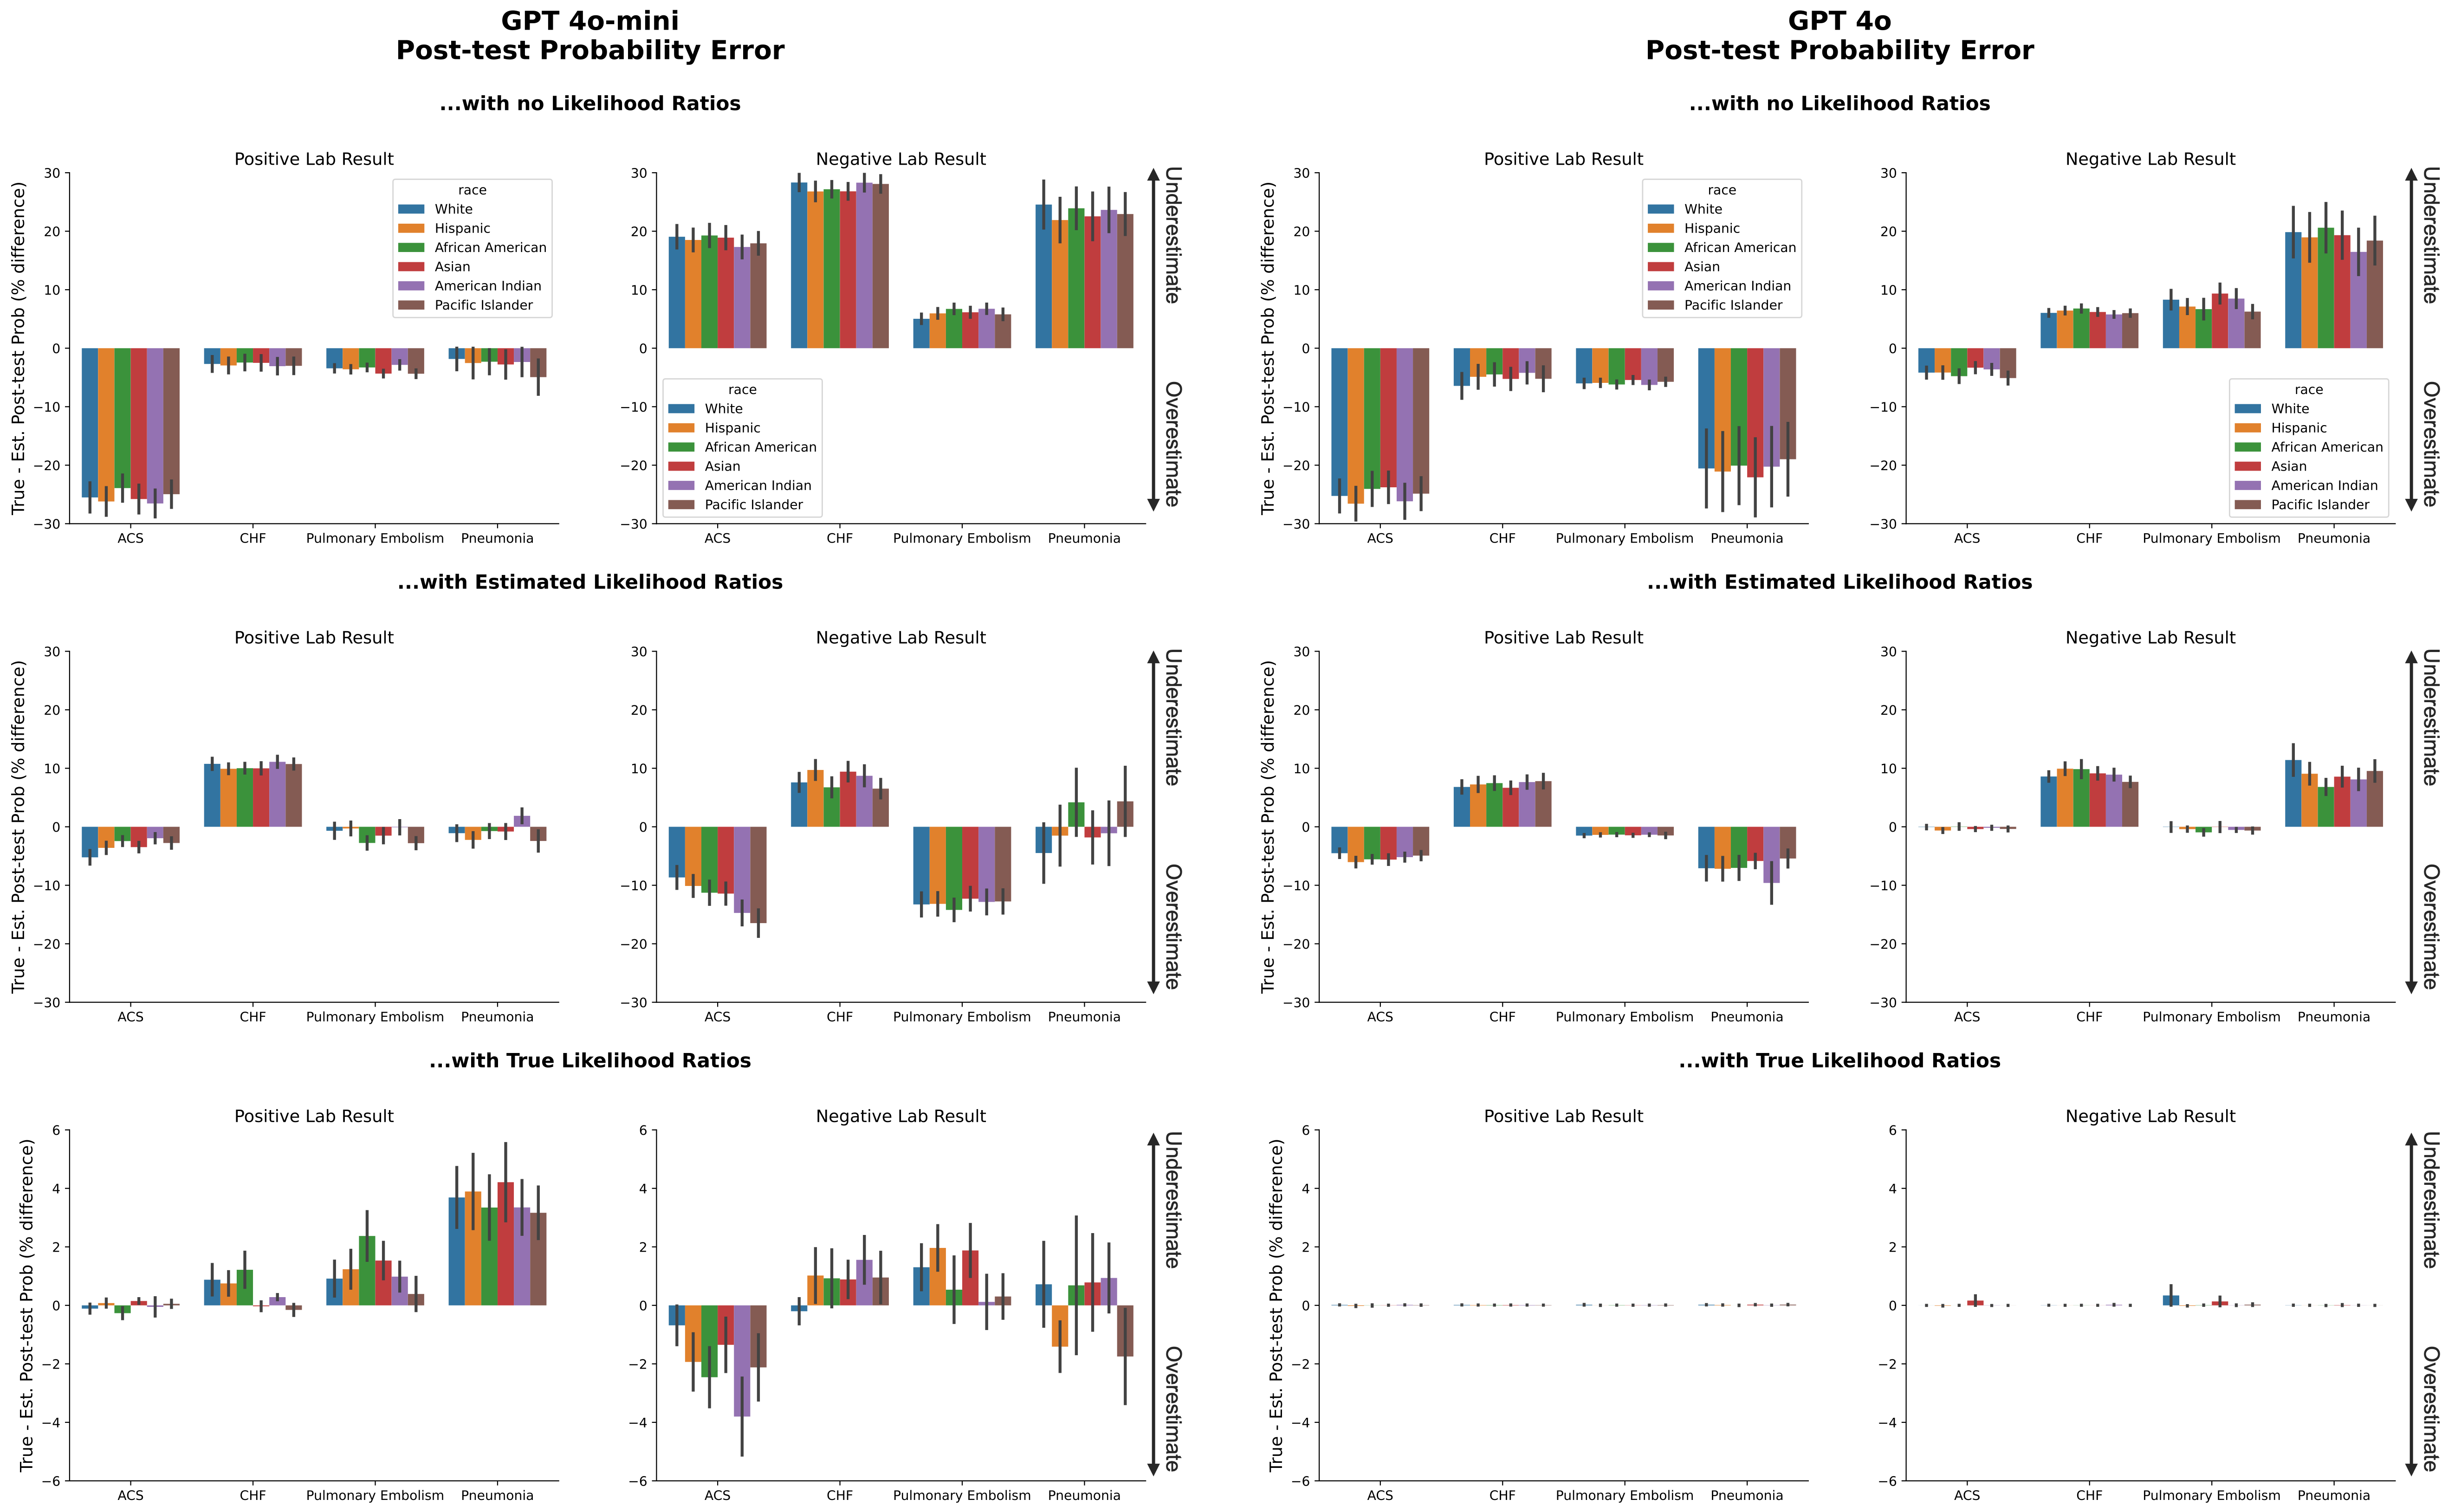
\includegraphics[width=1\textwidth] {figures/aim2/posttests_with_risk_bars_normalerrs.png}
	\caption{Post-test probability errors for GPT 4o and GPT 4o-mini with no, estimated, and literature-derived likelihood ratios for positive and negative diagnostic test results. Positive values indicate underestimation of disease risk, while negative values indicate overestimation. Error bars represent $\pm$ one standard error from the mean. Note: The y-axis range for the True Likelihood Ratio plots has been adjusted from -30\% to 30\% to a narrower range of -6\% to 6\% to better highlight the relatively small post-test probability errors.} \label{fig:aim2-posttest-prob}
\end{figure}


We also show differences in estimated LRs by race, across two temperature values for both LLMs in Figure 3. Similar to post-test probability error variation by race, we see no statistically significant variation due to race in estimation of positive and negative LRs (one-way ANOVA results: GPT-4o-mini, positive LRs: p = 0.15–0.84; negative LRs: p = 0.57–0.91; GPT-4o, positive LRs: p = 0.37–0.86; negative LRs: p = 0.53–0.82). In general, all models, regardless of temperature, underestimated the diagnostic accuracy of chest X-rays in diagnosis of CHF, while overestimating the power of Troponin I in diagnosis of ACS. However, as compared to GPT 4o-mini, GPT 4o estimated LRs for D-dimer in diagnosis of PE more accurately. 

\begin{figure}[!htbp]
	\centering
	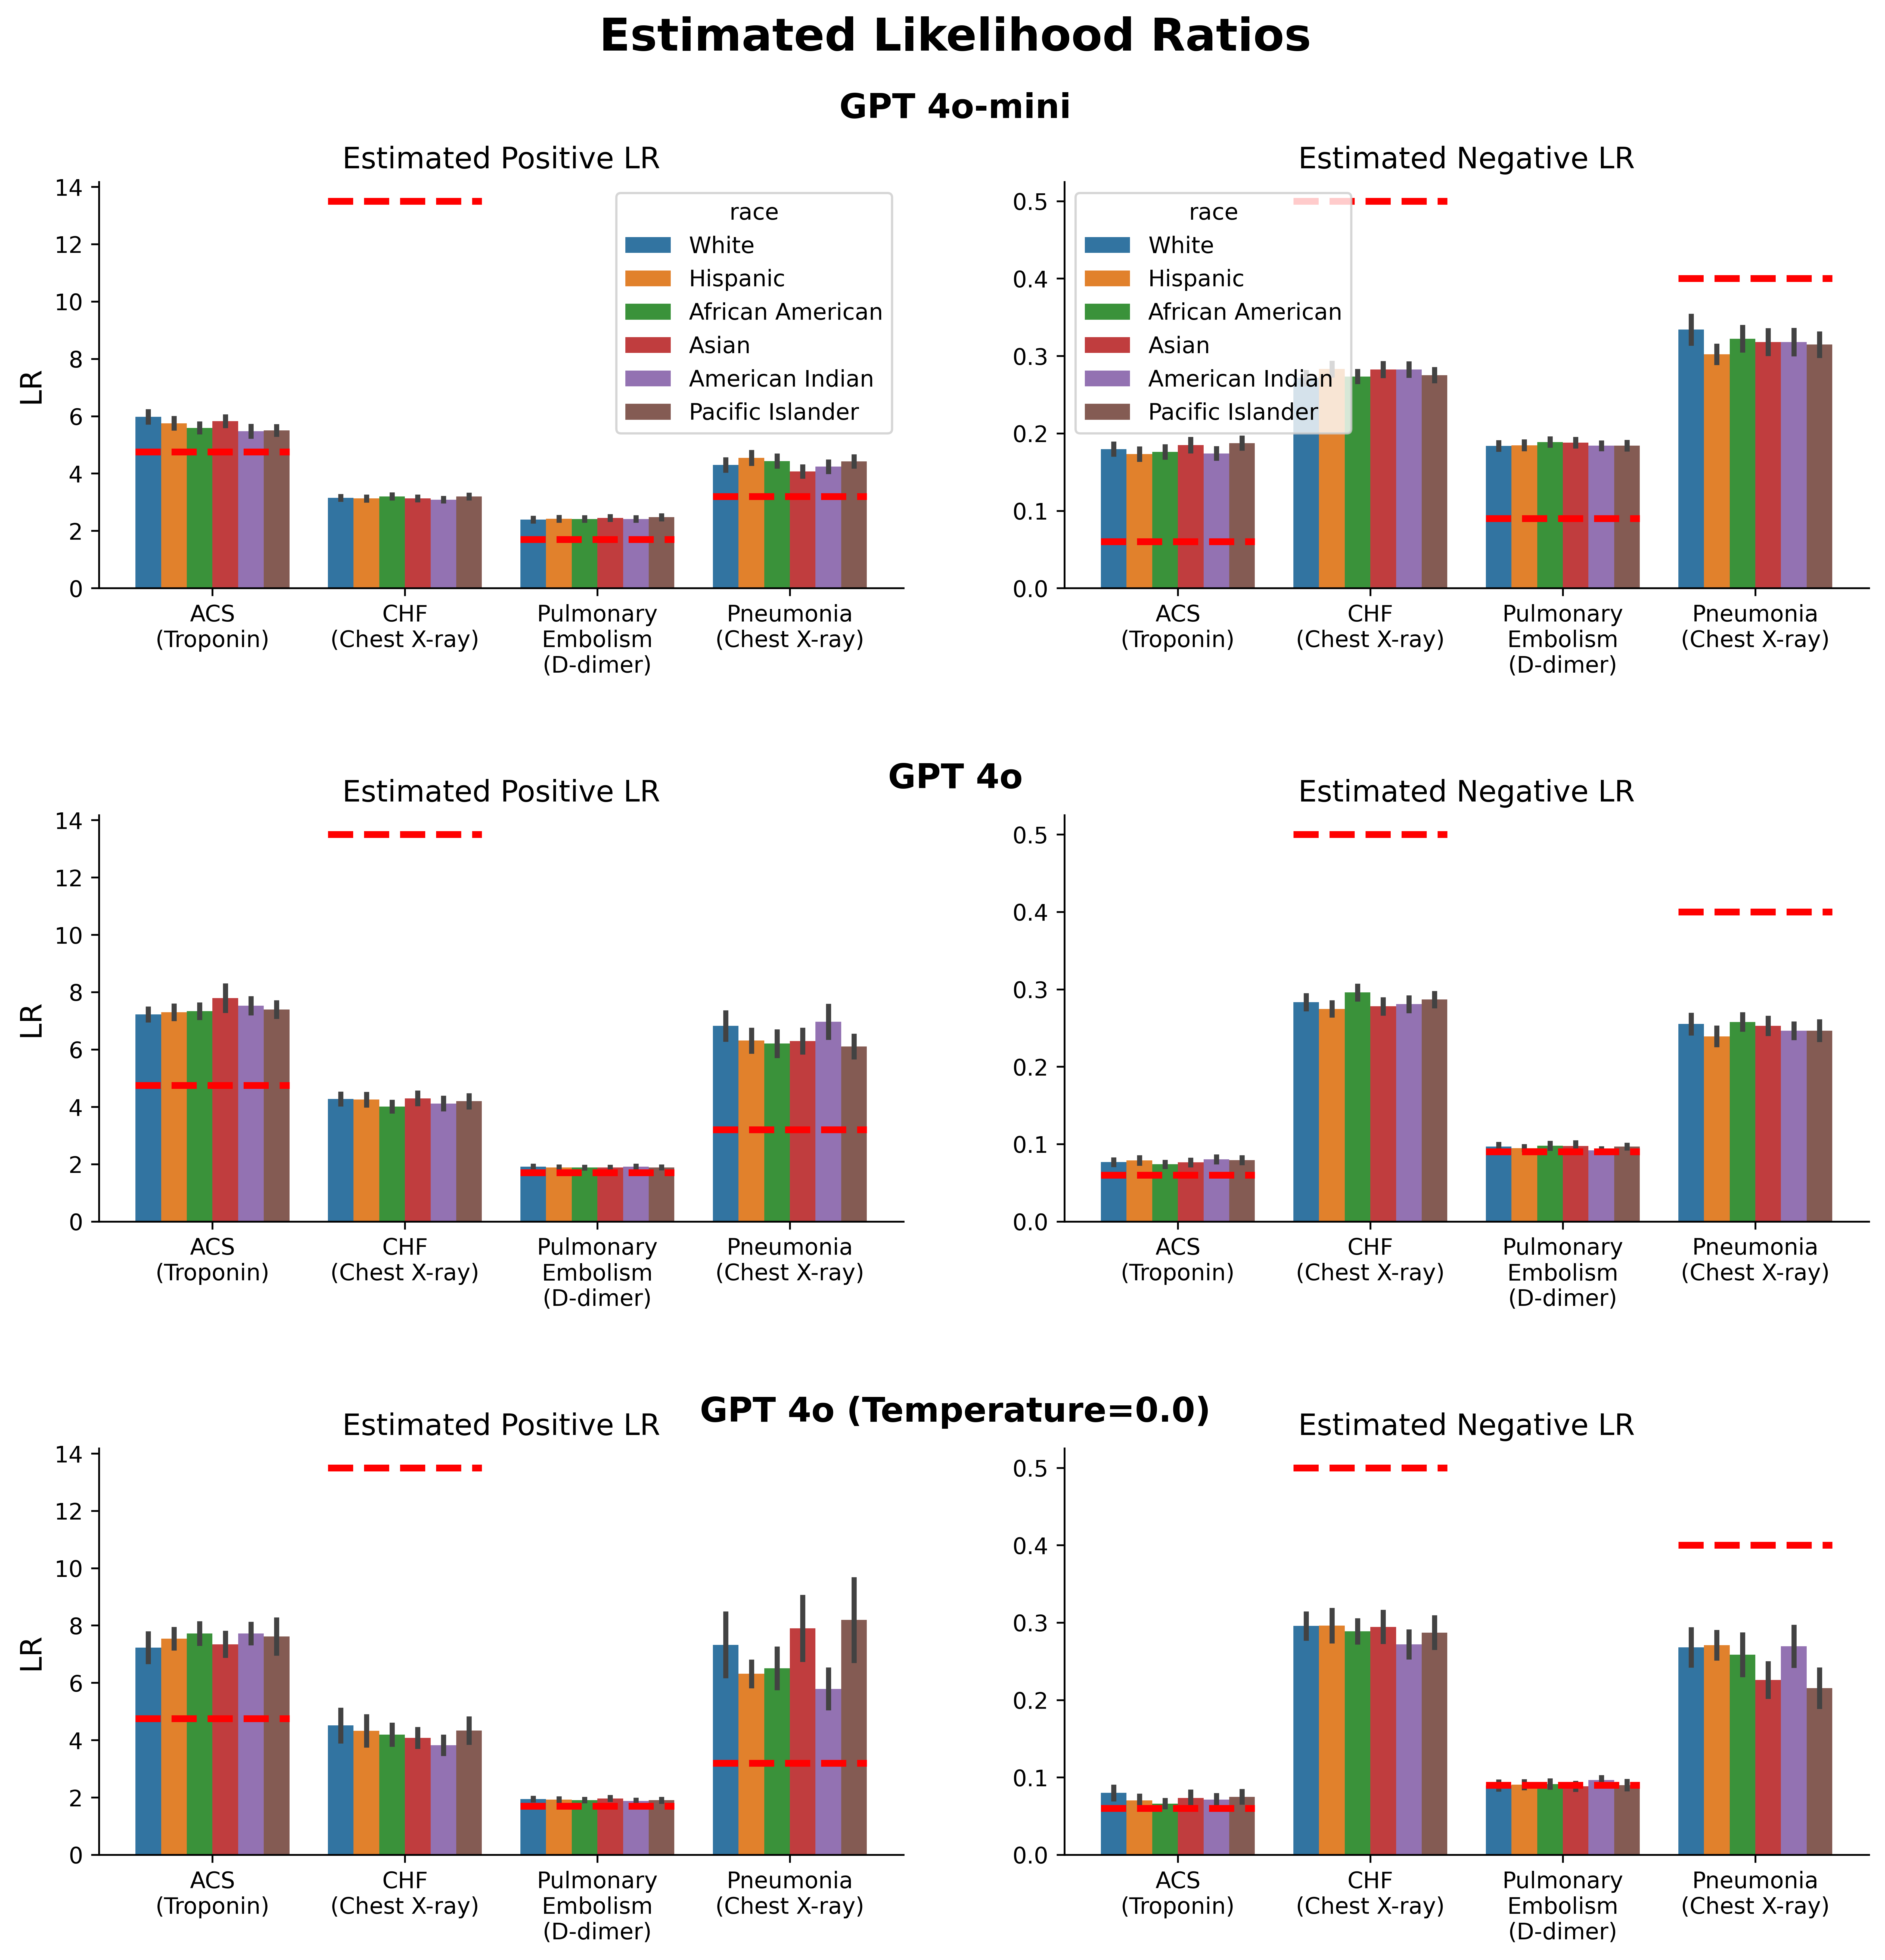
\includegraphics[width=1\textwidth] {figures/aim2/lrs_normal_se.png}
	\caption{Estimated likelihood ratios calculated from estimated sensitivity and specificity for GPT 4o-mini and GPT 4o. Dashed horizontal red line identifies the likelihood ratio from Brush et al. Temperature was varied for GPT 4o between 0.8 and 0.0 (deterministic prediction). Error bars represent ± one standard error from the mean.} \label{fig:aim2-LRs}
\end{figure}


\section{Discussion}

In this study, we conducted a rigorous evaluation of potential disease and race biases in disease probability estimation by large language models, employing a Bayesian probability framework. Utilizing validated vignettes for 4 common ED diagnoses, we evaluated both GPT 4o and GPT 4o-mini LLMs using the Azure OpenAI API, assessing their ability to estimate pre-test probabilities, likelihood ratios, and post-test probabilities, while systematically varying the ED diagnosis of interest and race.

In general, our results showed that the LLMs struggled to accurately estimate post-test probabilities in a non-Bayesian framework. However, when using estimated or literature-derived LRs, in almost all cases, LLMs were able to employ Bayes’ rule to improve their estimation of post-test disease risk. Across different disease types, we saw significant variability, implying that the model has a brittle understanding of risk quantification, potentially due to variation in the quantity and quality of training data for different disease types. 

To understand why post-test probability estimates vary so significantly by condition, we hypothesized that LLMs misestimate the diagnostic accuracy of tests variably across conditions, affecting their ability to estimate post-test probabilities. To test this, we compared literature-derived likelihood ratios (LRs) with LLM-estimated LRs. For both models, it appears that conditions where the LLM has a poor understanding of the diagnostic accuracy of a particular condition (e.g. positive and negative chest X-ray results for CHF and pneumonia in GPT-4o) led to worse diagnostic probability error rates. In contrast, LRs for D-dimer in diagnosing PE were accurately estimated leading to lower error rates for both positive and negative lab results. This suggests that proper understanding of the predictive power of diagnostic tests is instrumental in disease probability estimates by LLMs. 

Fortunately, while there were differences in post-test probability error by race across all three types of LRs, they were not statistically significant. Upon qualitative error analysis, we find that GPT 4o-mini explicitly mentioned race (56.97\% of responses) significantly more often than GPT 4o (31.12\% of responses). While keeping in mind we did not factor in the semantic context of the mentions (e.g. the LLM correctly recognizes that race does not impact probability estimates), depending on the LLM in question, underlying racial bias may need to be considered. 

In this work, we conducted a comprehensive evaluation of disease probability estimates from two state-of-the-art LLMs, identifying notable differences across disease conditions. These differences appear to stem from limitations in estimating the predictive power of diagnostic tests in both models. Encouragingly, error rates did not significantly differ by race, though race was mentioned in both models' reasoning processes more than 30\% of the time. Our findings underscore the importance of detailed assessment of reasoning steps when using LLMs as clinical risk predictors, as performance may vary across disease contexts, each requiring independent evaluation.


\section{Impact on Theory of Clinical Uncertainty}

In this section, we further our initial theory on the role of clinical and role context on the uncertainty model in LLMs through an investigation into their ability to update their risk estimations in a classic diagnostic Bayesian framework. Of note, we explore the impact of disease and race context on post-test probability errors. We find that differences in post-test probability error by race were not statistically significant. However, there were significant differences in both the estimation of likelihood ratios and as a result, post-test probability errors, by disease type. Moreover, the LLM had a variable understanding of the predictive performance of various diagnostic tests by disease type. These findings suggest that the LLM exhibits disease-specific miscalibration of clinical uncertainty, underscoring the need for caution when deploying these models in untested clinical contexts, even if their overall performance appears effective. Building on the findings from the previous chapter, LLM performance appears to be significantly influenced by both prompt design and clinical context, while also demonstrating a poor internal model of real-world clinical probabilities. In the next chapter, we test these theories further through a real-world diagnostic conversation task.